\documentclass[12pt]{article}

\usepackage{graphicx}
\usepackage{indentfirst} % garante que a primeira linha terá identação.
\usepackage{listings}
\usepackage{xcolor}
\usepackage{hyperref}       % Permite o uso de hyperlinks no texto, com um link clicável

\definecolor{codegreen}{rgb}{0,0.6,0}
\definecolor{codegray}{rgb}{0.5,0.5,0.5}
\definecolor{codepurple}{rgb}{0.58,0,0.82}
\definecolor{backcolour}{rgb}{0.95,0.95,0.92}

\lstdefinestyle{mystyle}{
    backgroundcolor=\color{backcolour},   
    commentstyle=\color{codegreen},
    keywordstyle=\color{magenta},
    numberstyle=\tiny\color{codegray},
    stringstyle=\color{codepurple},
    basicstyle=\ttfamily\footnotesize,
    breakatwhitespace=false,         
    breaklines=true,                 
    captionpos=b,                    
    keepspaces=true,                 
    numbers=left,                    
    numbersep=5pt,                  
    showspaces=false,                
    showstringspaces=false,
    showtabs=false,                  
    tabsize=2
}

\lstset{style=mystyle}
\newcommand{\blue}[1]{\textcolor{blue}{#1}}

\title{API Segura com Autenticação de Mensagens}
\author{Gabriel Henrique do Nascimento Neres \\ Arthur Diehl Barroso}
\date{\today}

\begin{document}
\maketitle

\begin{abstract}
    
    Esse trabalho aborda o desafio de assegurar a autenticidade e a integridade da dados transportados, propondo como objetivo o desenvolvimento de uma API RESTful segura, na qual cada requisição sensível inclui uma assinatura digital de sua carga útil (payload). Para isso, foi desenvolvido um protótipo cliente-servidor utilizando a linguagem de programação Java e o framework Quarkus. A camada de segurança foi implementada por meio da geração de um hash SHA-256 do corpo da mensagem, que é então assinado com um algoritmo RSA, utilizando um certificado digital autoassinado armazenado em uma keystore.
  \textbf{Palavras-chave}: API REST, Segurança Computacional, Assinatura Digital, Java, Quarkus.
\end{abstract}

\section{Introdução}

A arquitetura REST (Representational State Transfer) define um conjunto de restrições para a criação de sistemas de hipermídiam distribuídos. Uma API que adere a esse princípios conhecida como RESTful, é organizada em torno de recursos que são identificados por URLs únicas. A interação com esses recursos é realizada por meio dos métodos padrões do protocolo HTTP, como GET, POST e PUT. Uma característica fundamental dessa arquitetura é ser stateless, o que significa que cada requisição envidada do cliente para o servidor deve conter toda a informação necessária para ser processada, sem que o servidor precise manter um estado da sessão do cliente.


Embora essa arquitetura simplifique a comunicação cliente-servidor, o protocolo HTPP por si só não oferece garantias sobre a identidade do remetente ou a integridade dos dados na camada de aplicação. Em cenários que envolvem o envio de dados confidenciais ou comandos críticos, é essencial que seja adicionada uma camada de segurança que previna a manipulação ou a falsificação de requisições.

Este trabalho aborda esse problema através da implementação de uma API RESTful segura. O objetivo é aplicar uma assinatura digital na carga útil (payload) de cada requisição, garantindo assim a autenticidade (comprovação da identidade do remetente) e a integridade (não alteração de dados). O protótipo foi desenvolvido em Java com o framework Quarkus, dividido em um módulo Servidor, que expõe os endpoints, e um módulo Cliente, que consome esses endpoints e interage com uma interface web usada para testes.

\section{Arquitetura da Aplicação}

O sistema foi projetado seguindo uma arquitetura cliente-servidor, composta por dois módulos principais desenvolvidos em Java com o framework Quarkus:

\begin{itemize}
    \item \textbf{Módulo Servidor}: Funciona como a API REST principal. Foram expostos dois endpoints para manipulação de recursos:
    \begin{itemize}
        \item \textbf{POST /server/post}: Endpoint que recebe dados no corpo (payload) da requisição HTTP.
        \item  \textbf{GET /server/get/{body}}: Endpoint que recebe dados como um parâmetro na própria URL da requisição.
    \end{itemize}
    \item  \textbf{Módulo Cliente}: Atua como um intermediário que consome a API do Servidor. Este módulo também expõe uma API REST, projetada para ser consumida por uma interfaca web (HTML), simplificando a interação e os testes. É nesse módulo que a lógica de assinatura digital das requisições é executada antes de serem enviadas ao Servidor.
\end{itemize}

A segurança das requisições é centralizada na classe SignatureFilter no lado do Servidor. Esta classe funciona como um filtro que intercepta todas as chamadas recebidas, substituindo o comportamento padrão da aplicação para executar a lógica de verificação da assinatura antes de permitir que a requisição prossiga para os endpoints.

\section{Implementação da Camada de Segurança}

A segurança da API é baseada em um sistema de assinatura digital assimétrica (RSA) para garantir a autenticidade e a integridade de cada mensagem. Diferentemente de uma abordagem com chaves pré-compartilhadas, o cliente envia seu certificado digital junto com cada requisição, permitindo que o servidor utilize a chave pública contida nele para a verificação.

\subsection{Geração e Gerenciamento de Chaves}

Para o protótipo, foi gerado um certificado digital X.509 autoassinado, contendo um par de chaves RSA de 2048 bits. Esse certificado foi armazenado em um arquivo Java KeyStore (client-keystore.jks).

O acesso programático à keystore é realizado pela classe de utilitários CryptoUtils.java \ref{fig:CryptoUtils}. Ela é responsável por carregar a chave privada, usada pelo cliente para assinar os dados, e o certificado, que é enviado na requisição.

\begin{figure}[h]
    \centering
    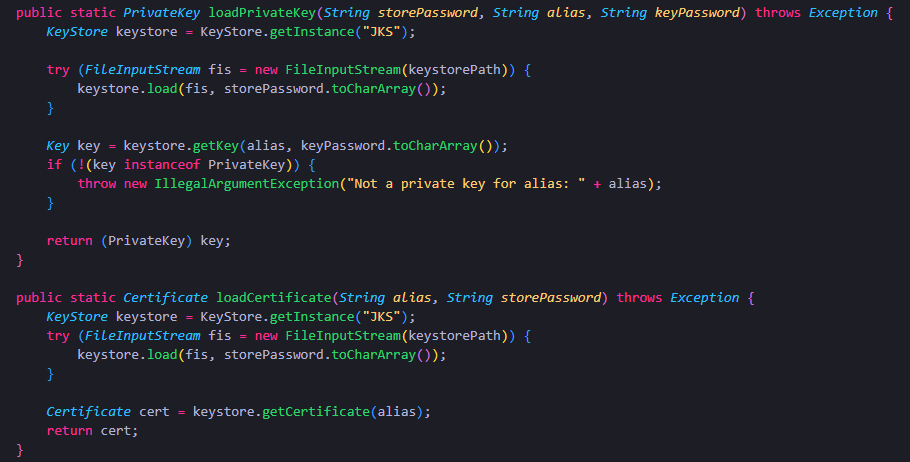
\includegraphics[width=0.8\linewidth]{Imagens/CryptoUtils.png}  
    \caption{Métodos da classe CryptoUtils para carregar a chave privada e o certificado da keystore.}
    \label{fig:CryptoUtils}
\end{figure}

\subsection{Fluxo da Requisição Segura}
O processo de assinatura e verificação é executado a cada chamada à API seguindo os seguites passos:
\begin{enumerate}
    \item \textbf{Assinatura}:
    \begin{itemize}
        \item \textbf{Seleção dos Dados}: Os dados a serem assinados são definidos com base no método HTTP. Para requisições POST, utiliza-se o próprio corpo (payload) da requisição. Para requisições GET, que não possuem corpo, constrói-se uma string canônica concatenando o nome do método e o caminho da requisição (ex: "GET - /server/get/meus-dados").
        \item \textbf{Geração da Assinatura}: Os dados selecionados são transformados em um hash com o algoritmo SHA-256, que é então criptografado com a chave privada do cliente via RSA. Este processo é encapsulado no método CryptoUtils.signData.
        \item \textbf{Montagem da Requisição}: O certificado do cliente e a assinatura digital gerada são codificados em Base64 e adicionados a dois cabeçalhos HTTP customizados: X-Certificate e X-Signature, respectivamente. A requisição é então enviada ao servidor.
    \end{itemize}
    \item \textbf{Verificação}:
    \begin{itemize}
        \item \textbf{Extração de Dados}: O filtro intercepta a requisição e extrai o conteúdo dos cabeçalhos X-Certificate e X-Signature. Se algum deles estiver ausente, a requisição é negada.

        \item \textbf{Validação do Certificado}: O certificado recebido é decodificado e sua validade é verificada com o método cert.checkValidity(). A chave pública é extraída do certificado validado.

        \item  \textbf{Reconstrução dos Dados}: O servidor reconstrói a mensagem original que foi assinada, seguindo a mesma lógica do cliente: para POST, lê o corpo da requisição; para GET, concatena o método e o caminho.

        \item \textbf{Verificação da Assinatura}: Com a chave pública, o servidor decriptografa a assinatura para obter o hash original. Este hash é comparado com um novo hash calculado a partir dos dados reconstruídos. Se os hashes corresponderem, a assinatura é válida (sig.verify()), e a requisição pode prosseguir. Caso contrário, ou se o certificado estiver expirado, a requisição é abortada com um status 403 Forbidden.


    \end{itemize}
\end{enumerate}

\section{Problemas observados}
Durante a implementação alguns problemas de segurança foram observados no protótipo final obtido. Os principais problemas observados foram:
\begin{itemize}
  \item A cada requisição é preciso obter os dados do certificado para a realização de assinatura da mensagem, deixando o processo muito mais lento;
  \item Falta de meios para as credenciais do usuário serem passadas a aplicação (cliente), sendo uma falha para a segurança do processo;
  \item Falta de confidenciabilidade da mensagem enviada;
\end{itemize}

\section{Código}
O código está disponível no github pelo link: \href{https://github.com/TheMasterGame0/Rest-Seguro}{https://github.com/TheMasterGame0/Rest-Seguro}

\end{document}